\documentclass[twocolumn]{article}

\usepackage{times}
\usepackage{fullpage}
\usepackage{stfloats}
\usepackage[font=small,skip=0pt]{caption}

% package to draw diagrams
\usepackage{tikz}
\usetikzlibrary{shapes.geometric}
\tikzstyle{data}=[draw,ellipse,minimum width=1cm,minimum height=0.5cm,align=center]
\tikzstyle{tool}=[draw,rectangle,minimum width=1cm,minimum height=0.5cm,align=center]

\pagestyle{empty}

\begin{document}

\pagenumbering{gobble}

\title{\vspace{-2cm}jpf-ctl: CTL Model Checking of Java Code}
\author{Parssa Khazra, Anto Nanah Ji, Matt Walker, Hongru Wang, and Franck van Breugel\\
Department of Electrical Engineering and Computer Science, York University, Toronto}
\date{\vspace{-0.5cm}}
\maketitle

Although several attempts have been made to extend \emph{Java PathFinder} (JPF) \cite{VHBPL03} to support model checking of linear temporal logic (LTL) \cite{P77}, we are not aware of any extension of JPF that provides \emph{computation tree logic} (CTL) \cite{CE81} model checking.  Our extension, named jpf-ctl, extends JPF so it can check whether a Java app satisfies a property expressed in CTL.  An overview of our tool can be found in Figure~\ref{figure:tool}.  In the remainder of this abstract, we briefly discuss the four components that we developed.

\begin{figure*}[b!]
\begin{center}
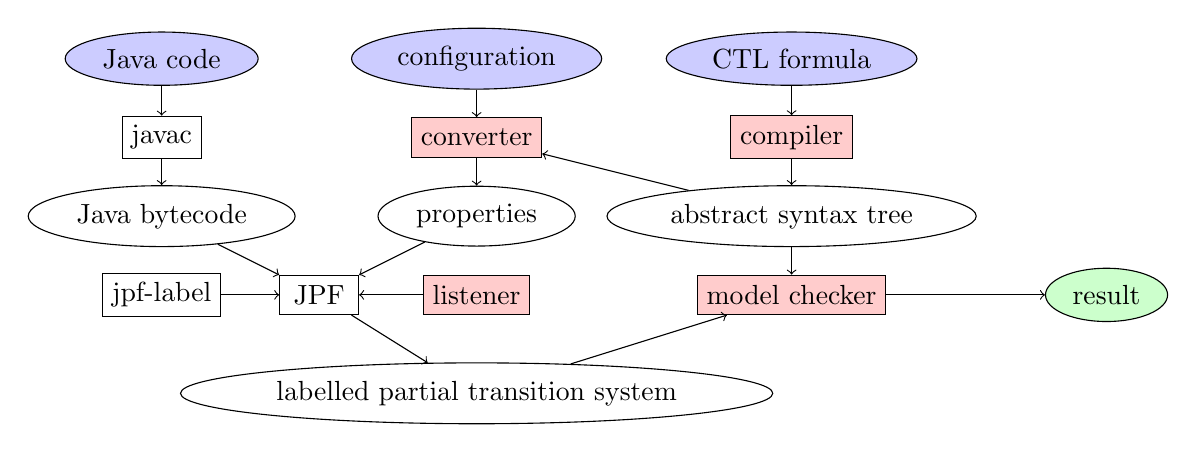
\begin{tikzpicture}
\node[data,fill=blue!20] (ctl) at (12,4) {CTL formula};
\node[tool,fill=red!20] (compiler) at (12,3) {compiler};
\node[data] (ast) at (12,2) {abstract syntax tree};

\node[data,fill=blue!20] (configuration) at (8,4) {configuration};
\node[tool,fill=red!20] (converter) at (8,3) {converter};

\node[data,fill=blue!20] (java) at (4,4) {Java code};
\node[tool] (javac) at (4,3) {javac};
\node[data] (bytecode) at (4,2) {Java bytecode};
\node[data] (properties) at (8,2) {properties};
\node[tool] (jpf) at (6,1) {JPF};
\node[tool] (jpf-label) at (4,1) {jpf-label};
\node[tool,fill=red!20] (jpf-ctl) at (8,1) {listener};
\node[data] (system) at (8,-0.25) {labelled partial transition system};

\node[tool,fill=red!20] (checker) at (12, 1) {model checker};
\node[data,fill=green!20] (result) at (16,1) {result};

\draw[->] (ctl)--(compiler);
\draw[->] (compiler)--(ast);

\draw[->] (java)--(javac);
\draw[->] (javac)--(bytecode);
\draw[->] (bytecode)--(jpf);
\draw[->] (properties)--(jpf);
\draw[->] (jpf-label)--(jpf);
\draw[->] (jpf-ctl)--(jpf);
\draw[->] (jpf)--(system);
\draw[->] (checker)--(result);

\draw[->] (configuration)--(converter);
\draw[->] (ast)--(converter);
\draw[->] (converter)--(properties);

\draw[->] (ast)--(checker);
\draw[->] (system)--(checker);
\end{tikzpicture}
\end{center}
\caption{The diagram provides an overview of the CTL model checking tool.  The ovals are data and the rectangles are tools.  The blue ovals are input.  The green ovals are output.  The red rectangles are the parts that we developed.}
\label{figure:tool}
\end{figure*}

\textbf{Compiler}  By means of ANTLR \cite{P13}, we generated a lexer and a parser.  We implemented an inheritance hierarchy of classes to represent the abstract syntax trees.  We used ANTLR's support of the visitor design pattern to transform the parse tree generated by the lexer and parser into an abstract syntax tree.

\textbf{Converter}  The converter extracts from the abstract syntax tree the atomic propositions that are used in the CTL formula.  Currently, our tool only supports static boolean fields as atomic propositions.  The converter combines this information with other configuration data, such as JPF's classpath and native classpath, into an application properties file that is used by JPF.

\textbf{Listener}  Our listener generates a \emph{partial} transition system that models the Java code.  Such a partial transition system differs from an ordinary transition system in that some states may be designated as partially explored.  States may only be partially explored as JPF runs out of memory or takes too much time.  The extension jpf-label \cite{F20} allows us to label the states with atomic propositions.

\textbf{Model checker}  Given a labelled partial transition system and the abstract syntax tree of a CTL formula, we implemented a model checking algorithm to determine whether the system satisfies the formula.  Like the algorithm presented in \cite{BG99} to deal with partial systems, our algorithm uses a three-valued logic and computes a pessimistic interpretation and an optimistic interpretation.  Given a CTL formula, we approximate the set of states of the partial system that satisfy the formula no matter how the partial system is extended.  Furthermore, we also approximate the set of states of the partial system for which there exists an extension that satisfies the formula.  To compute these pessimistic and optimistic approximations of the satisfaction set of a formula, we use variations on the standard algorithm to compute the satisfaction set of a formula (see, for example, \cite[Section~6.4]{BK08}) and prove our algorithm correct.  

Given a CTL formula~$\varphi$, let us denote the pessimistic approximation of the satisfaction set of $\varphi$ by $P_{\varphi}$ and the optimistic one by $O_{\varphi}$.  If the initial state of the labelled partial transition system belongs to $P_{\varphi}$ then we can conclude that the system satisfies $\varphi$.  In this case, the result of the model checker is a witness that illustrates that the partial system satisfies $\varphi$.  If the initial state of the labelled partial transition system does not belong to $O_{\varphi}$ then we can conclude that the system does not satisfy  $\varphi$.  In this case, the result of the model checker is a counterexample that illustrates that the partial system does not satisfy $\varphi$.  Otherwise, the initial state of the labelled partial transition system does not belong to $P_{\varphi}$ but belongs to $O_{\varphi}$, since $P_{\varphi} \subseteq O_{\varphi}$.  This third value corresponds to the case in which we cannot conclude whether the partial system satisfies $\varphi$.

\newpage

\bibliographystyle{plain}
\bibliography{abstract}

\end{document}
